% =====================================================================
% SECTION 1: DATA UNDERSTANDING AND PREPARATION (COMPACT ~4.5 PAGES)
% Requires in preamble: \usepackage{booktabs,graphicx,tabularx,amsmath,amssymb,caption,subcaption}
% Place figures in report/figures/:
%   - fig1_1_histograms_compact.png
%   - fig1_2_categorical_combined.png
%   - fig1_3_boxplots_outliers_compact.png
%   - fig1_4_pairplot_compact.png
%   - fig1_5_spearman_heatmap_compact.png
% =====================================================================

\section{Data Understanding and Preparation}
\label{sec:understanding}

\subsection{Data semantics}
\label{sec:semantics}
The \emph{Seller-Level Vehicle Listings Dataset} comprises 13,843 records and 33 attributes (1 identifier, 24 numerical, and 8 categorical), where each row aggregates the vehicle inventory and listing activity of a unique seller (\texttt{sp\_id}). Numerical attributes capture seller-level medians for pricing, mileage, vehicle specifications, and title-risk proportions (\texttt{pct\_*}), while categorical attributes record the seller's modal vehicle characteristics, market positioning, and the ordinal classification target \texttt{seller\_rating\_class} (\texttt{low}, \texttt{medium}, \texttt{high}), as detailed in Table~\ref{tab:semantics}.

\begin{table}[htbp]
  \centering
  \caption{Semantic description of the 33 dataset variables.}
  \label{tab:semantics}
  \footnotesize
  \renewcommand{\arraystretch}{0.92}
  \begin{tabular}{llll}
    \toprule
    \textbf{Feature Name} & \textbf{Description} & \textbf{Datatype} & \textbf{Msrmt Scale} \\
    \midrule
    \texttt{sp\_id} & Unique identifier of the seller/dealer & float64 & Identifier \\
    \texttt{n\_listings} & Total number of vehicle listings & int64 & Numerical \\
    \texttt{price\_median} & Median advertised price of vehicles (USD) & float64 & Numerical \\
    \texttt{savings\_amount\_median} & Median advertised savings amount (USD) & float64 & Numerical \\
    \texttt{daysonmarket\_median} & Median days vehicles remained on market & float64 & Numerical \\
    \texttt{mileage\_median} & Median vehicle mileage (miles) & float64 & Numerical \\
    \texttt{year\_median} & Median vehicle model year & float64 & Numerical \\
    \texttt{vehicle\_age\_median} & Median vehicle age at listing time (years) & float64 & Numerical \\
    \texttt{owner\_count\_median} & Median number of previous vehicle owners & float64 & Numerical \\
    \texttt{horsepower\_median} & Median vehicle horsepower (HP) & float64 & Numerical \\
    \texttt{engine\_displacement\_median} & Median vehicle engine displacement (cc) & float64 & Numerical \\
    \texttt{city\_fuel\_economy\_median} & Median city fuel economy (MPG) & float64 & Numerical \\
    \texttt{highway\_fuel\_economy\_median} & Median highway fuel economy (MPG) & float64 & Numerical \\
    \texttt{back\_legroom\_median} & Median rear-seat legroom (inches) & float64 & Numerical \\
    \texttt{front\_legroom\_median} & Median front-seat legroom (inches) & float64 & Numerical \\
    \texttt{fuel\_tank\_volume\_median} & Median fuel tank capacity (gallons) & float64 & Numerical \\
    \texttt{height\_median} & Median vehicle height (inches) & float64 & Numerical \\
    \texttt{length\_median} & Median vehicle length (inches) & float64 & Numerical \\
    \texttt{width\_median} & Median vehicle width (inches) & float64 & Numerical \\
    \texttt{pct\_isCab} & Proportion of vehicles previously used as cabs & float64 & Numerical \\
    \texttt{pct\_is\_new} & Proportion of vehicles classified as new & float64 & Numerical \\
    \texttt{pct\_salvage} & Proportion of vehicles with salvage status & float64 & Numerical \\
    \texttt{pct\_theft\_title} & Proportion of vehicles with theft titles & float64 & Numerical \\
    \texttt{n\_listing\_days} & Distinct calendar days with observed listings & int64 & Numerical \\
    \texttt{listing\_span\_days} & Span in days between earliest and latest listing & int64 & Numerical \\
    \texttt{dominant\_body\_type} & Most frequent vehicle body type & str & Categorical \\
    \texttt{dominant\_fuel\_type} & Most frequent fuel type & str & Categorical \\
    \texttt{dominant\_transmission} & Most frequent transmission type & str & Categorical \\
    \texttt{dominant\_wheel\_system} & Most frequent drivetrain configuration & str & Categorical \\
    \texttt{dominant\_listing\_color} & Most frequent exterior color & str & Categorical \\
    \texttt{franchise\_status} & Franchise status (franchise, independent) & str & Categorical \\
    \texttt{new\_used\_profile} & Inventory composition (used\_only, mixed, new\_only) & str & Categorical \\
    \texttt{seller\_rating\_class} & Discretized target rating (low, medium, high) & str & Ordinal \\
    \bottomrule
  \end{tabular}
\end{table}

\subsection{Distribution of variables and statistics}
\label{sec:distribution}

\subsubsection{Summary of statistics}
Table~\ref{tab:stats} reports the descriptive statistics for all 24 numerical attributes, revealing three key structural properties. First, feature magnitudes vary across five orders of scale---from bounded proportions (\texttt{pct\_*} $\in [0, 1]$) and cabin dimensions (\texttt{height\_median} mean $65.15\text{ in}$) to \texttt{price\_median} (up to \$236,438) and \texttt{mileage\_median} (up to $238,541\text{ mi}$)---requiring standardisation prior to distance-based modelling. Second, volume, pricing, and adverse-history indicators exhibit severe right skewness ($\text{Skewness} > 1$) and heavy tails (high kurtosis), most notably \texttt{pct\_theft\_title} ($\text{Skew} = 14.11, \text{Kurt} = 427.34$), \texttt{pct\_salvage} ($\text{Skew} = 10.34$), \texttt{daysonmarket\_median} ($\text{Skew} = 8.75$), and \texttt{n\_listings} ($\text{Skew} = 5.25$, where the mean of $118.10$ far exceeds the median of $70.00$). Conversely, \texttt{year\_median} ($\text{Skew} = -2.25$) and \texttt{back\_legroom\_median} ($\text{Skew} = -3.53$) are left-skewed. Third, while most attributes are nearly complete, \texttt{engine\_displacement\_median} lacks 3,393 records ($24.51\%$), and sparse risk ratios (\texttt{pct\_salvage}, \texttt{pct\_theft\_title}) yield $\text{IQR} = 0$ because over $84\%$ of sellers have a zero median.

\begin{table}[htbp]
  \centering
  \caption{Summary statistics for the 24 numerical variables (identifier excluded).}
  \label{tab:stats}
  \scriptsize
  \renewcommand{\arraystretch}{0.92}
  \setlength{\tabcolsep}{3.5pt}
  \begin{tabular}{lrrrrrrrrrrrr}
    \toprule
    \textbf{Variable} & \textbf{Count} & \textbf{Mean} & \textbf{Std} & \textbf{Min} & \textbf{25\%} & \textbf{50\%} & \textbf{75\%} & \textbf{Max} & \textbf{Missing} & \textbf{Skew} & \textbf{Kurtosis} & \textbf{IQR} \\
    \midrule
    \texttt{n\_listings} & 13843 & 118.10 & 137.06 & 5.00 & 25.00 & 70.00 & 168.00 & 4959.00 & 0 & 5.25 & 120.32 & 143.00 \\
    \texttt{price\_median} & 13843 & 23106.14 & 14365.07 & 1699.00 & 12495.00 & 22385.00 & 29888.00 & 236438.00 & 0 & 3.45 & 34.14 & 17393.00 \\
    \texttt{savings\_amount\_median} & 13843 & 446.21 & 519.46 & 0.00 & 0.00 & 358.00 & 734.00 & 9333.00 & 0 & 2.40 & 18.30 & 734.00 \\
    \texttt{daysonmarket\_median} & 13843 & 49.15 & 56.06 & 0.00 & 26.00 & 36.00 & 51.00 & 1987.00 & 0 & 8.75 & 168.60 & 25.00 \\
    \texttt{mileage\_median} & 13842 & 51463.27 & 51845.46 & 0.00 & 25.00 & 33596.50 & 96915.75 & 238541.00 & 1 & 0.68 & -0.77 & 96890.75 \\
    \texttt{year\_median} & 13843 & 2015.95 & 4.72 & 1960.00 & 2013.00 & 2017.00 & 2020.00 & 2021.00 & 0 & -2.25 & 14.09 & 7.00 \\
    \texttt{vehicle\_age\_median} & 13842 & 4.08 & 4.63 & 0.00 & 0.00 & 3.00 & 7.00 & 60.00 & 1 & 2.32 & 14.98 & 7.00 \\
    \texttt{owner\_count\_median} & 13804 & 1.43 & 0.62 & 1.00 & 1.00 & 1.00 & 2.00 & 6.00 & 39 & 1.30 & 1.35 & 1.00 \\
    \texttt{horsepower\_median} & 13837 & 240.90 & 56.99 & 78.00 & 188.00 & 243.00 & 283.00 & 630.00 & 6 & 0.85 & 2.05 & 95.00 \\
    \texttt{engine\_displacement\_median} & 10450 & 2925.08 & 808.08 & 1200.00 & 2400.00 & 2500.00 & 3500.00 & 6800.00 & 3393 & 1.29 & 2.77 & 1100.00 \\
    \texttt{city\_fuel\_economy\_median} & 13827 & 20.65 & 3.96 & 10.00 & 18.00 & 20.00 & 22.00 & 126.00 & 16 & 8.10 & 185.87 & 4.00 \\
    \texttt{highway\_fuel\_economy\_median} & 13827 & 27.88 & 3.98 & 15.00 & 25.00 & 27.50 & 30.00 & 105.00 & 16 & 3.88 & 66.79 & 5.00 \\
    \texttt{back\_legroom\_median} & 13824 & 37.71 & 1.57 & 0.00 & 36.80 & 37.80 & 38.60 & 47.50 & 19 & -3.53 & 77.81 & 1.80 \\
    \texttt{front\_legroom\_median} & 13836 & 41.89 & 0.77 & 36.60 & 41.30 & 41.80 & 42.20 & 67.00 & 7 & 3.49 & 88.62 & 0.90 \\
    \texttt{fuel\_tank\_volume\_median} & 13836 & 18.35 & 2.93 & 7.15 & 16.40 & 18.25 & 19.20 & 52.00 & 7 & 1.83 & 7.33 & 2.80 \\
    \texttt{height\_median} & 13837 & 65.15 & 4.95 & 46.85 & 61.60 & 66.00 & 68.00 & 107.50 & 6 & 0.18 & 0.91 & 6.40 \\
    \texttt{length\_median} & 13837 & 191.10 & 10.25 & 151.00 & 184.60 & 189.80 & 192.70 & 282.30 & 6 & 2.18 & 7.59 & 8.10 \\
    \texttt{width\_median} & 13837 & 77.02 & 4.97 & 65.70 & 72.90 & 75.55 & 80.00 & 105.90 & 6 & 1.06 & 1.56 & 7.10 \\
    \texttt{pct\_isCab} & 13816 & 0.16 & 0.16 & 0.00 & 0.05 & 0.12 & 0.21 & 1.00 & 27 & 2.04 & 5.91 & 0.17 \\
    \texttt{pct\_is\_new} & 13843 & 0.27 & 0.32 & 0.00 & 0.00 & 0.00 & 0.59 & 1.00 & 0 & 0.55 & -1.38 & 0.59 \\
    \texttt{pct\_salvage} & 13816 & 0.01 & 0.06 & 0.00 & 0.00 & 0.00 & 0.00 & 1.00 & 27 & 10.34 & 119.82 & 0.00 \\
    \texttt{pct\_theft\_title} & 13816 & 0.00 & 0.02 & 0.00 & 0.00 & 0.00 & 0.00 & 0.76 & 27 & 14.11 & 427.34 & 0.00 \\
    \texttt{n\_listing\_days} & 13843 & 46.32 & 33.72 & 1.00 & 18.00 & 39.00 & 68.00 & 272.00 & 0 & 0.98 & 0.95 & 50.00 \\
    \texttt{listing\_span\_days} & 13843 & 405.59 & 282.37 & 0.00 & 223.00 & 362.00 & 508.00 & 3553.00 & 0 & 2.15 & 9.00 & 285.00 \\
    \bottomrule
  \end{tabular}
\end{table}

\subsubsection{Distribution via histograms}
Figure~\ref{fig:histograms} illustrates the distributions of the six core attributes governing seller scale, pricing, turnover, and inventory age. Operational scale (\texttt{n\_listings}), pricing (\texttt{price\_median}), and turnover time (\texttt{daysonmarket\_median}) follow heavily right-skewed distributions: the vast majority of dealers list fewer than 500 vehicles (median 70) and clear inventory within 200 days (median 36 days), whereas a sparse right tail extends to 4,959 listings and 1,987 days. Inventory composition exhibits strong structural polarization: \texttt{pct\_is\_new} and \texttt{mileage\_median} are distinctly bimodal, separating pure used-car dealers (\texttt{pct\_is\_new = 0}, median mileage around $30\text{k--}100\text{k mi}$) from franchise new-car dealers (\texttt{mileage\_median} near $0\text{ mi}$). Conversely, \texttt{year\_median} is strongly left-skewed ($\text{Skew} = -2.25$), concentrated in 2013--2020 with a long tail of classic-car sellers reaching 1960. Among the remaining unplotted attributes, \texttt{owner\_count\_median} concentrates tightly at 1--2 previous owners, while physical dimensions (\texttt{height\_median}, \texttt{length\_median}, \texttt{front\_legroom\_median}, \texttt{fuel\_tank\_volume\_median}) form narrow, high-kurtosis peaks around standard passenger-vehicle specifications.

\begin{figure}[htbp]
  \centering
  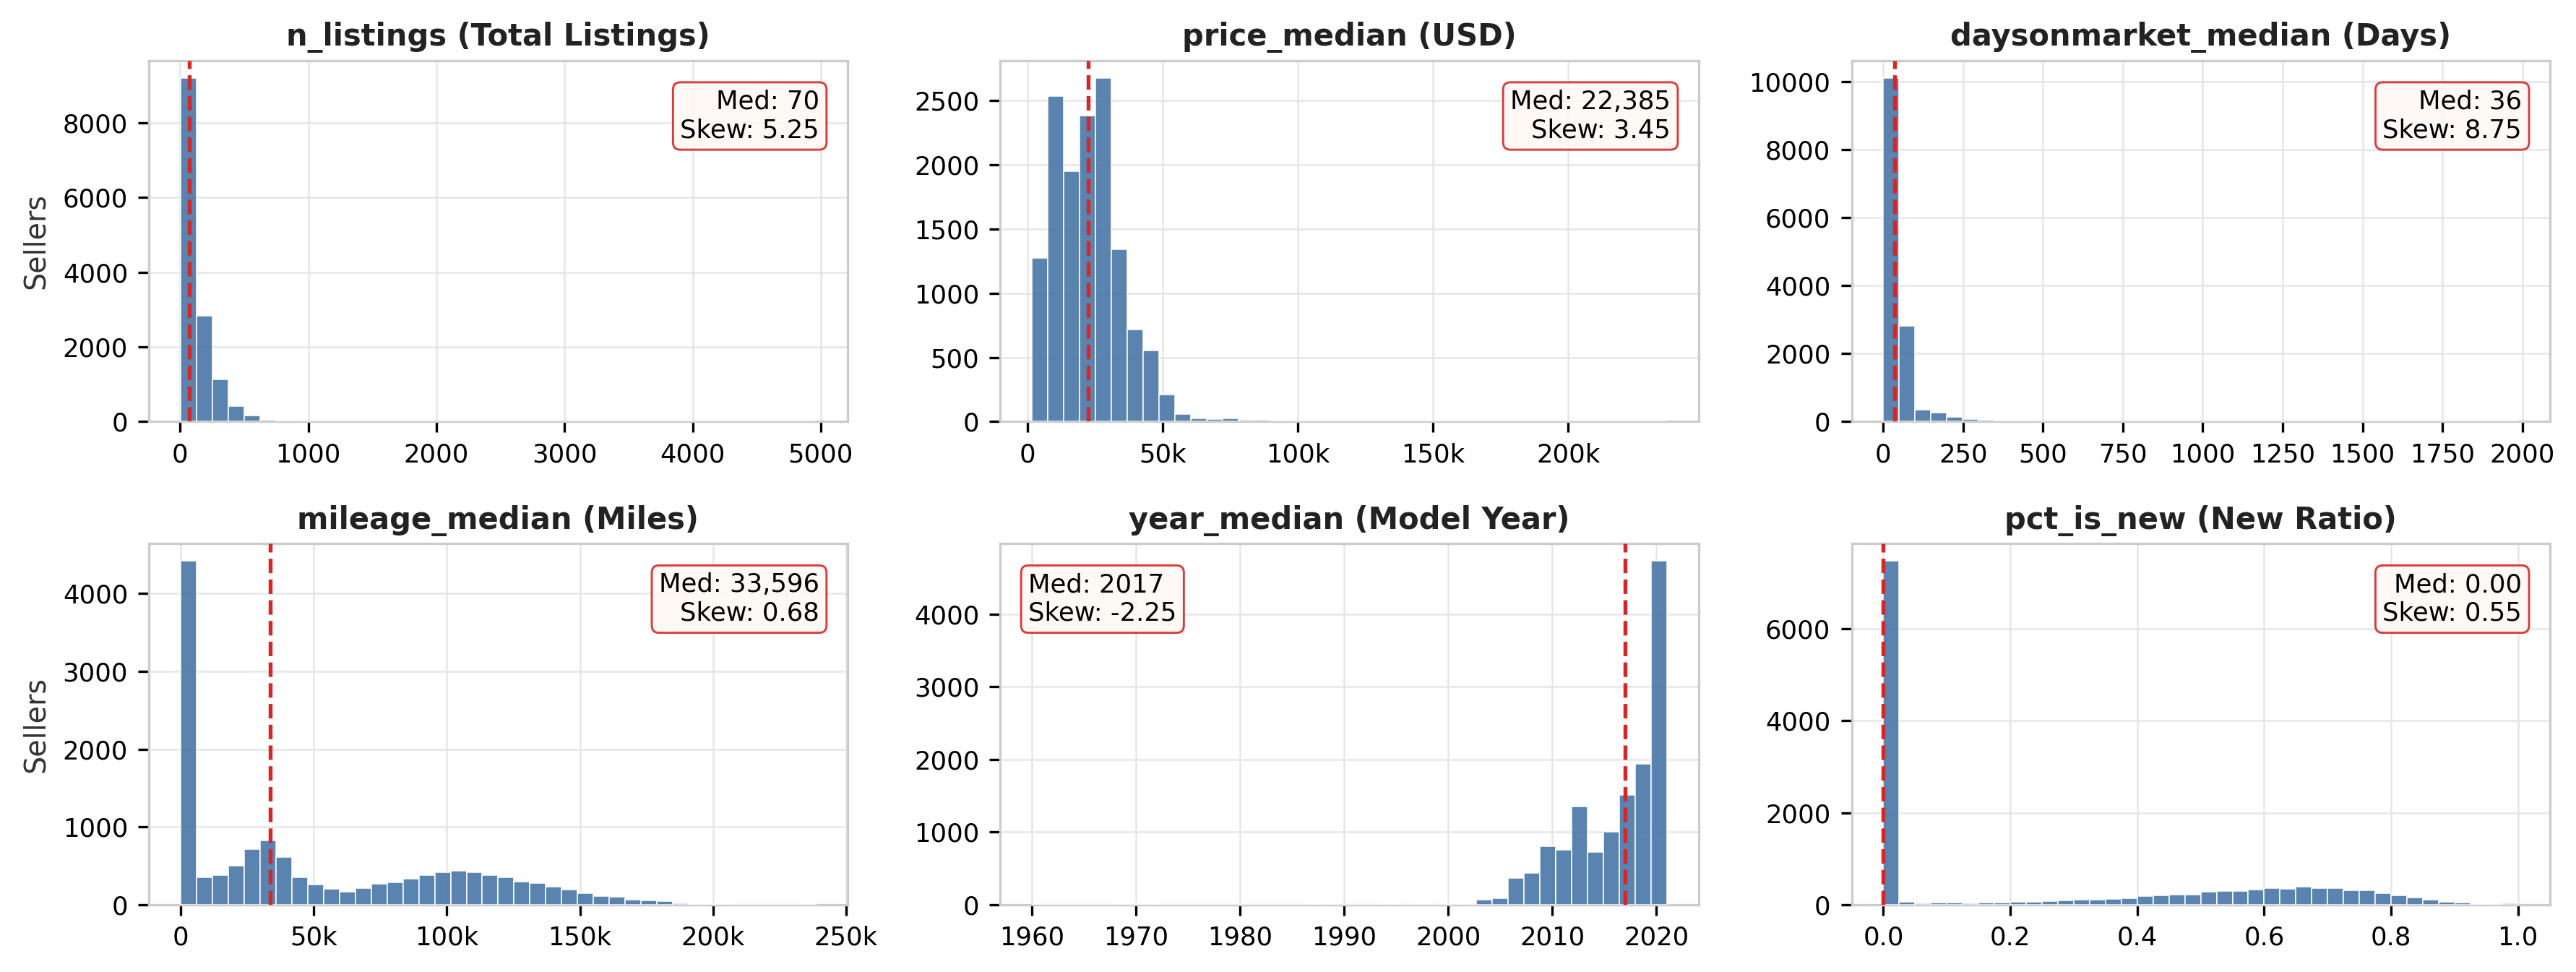
\includegraphics[width=0.96\textwidth]{figures/fig1_1_histograms_compact.png}
  \caption{Histograms of the six core numerical attributes with median lines and skewness statistics.}
  \label{fig:histograms}
\end{figure}

\subsubsection{Distribution of categorical features}
Figure~\ref{fig:categorical} summarises the six most informative categorical distributions. Among low-cardinality variables (top row), the target \texttt{seller\_rating\_class} is moderately imbalanced---led by \emph{medium} ($54.7\%$), followed by \emph{high} ($26.6\%$) and \emph{low} ($18.6\%$)---whereas market structure is evenly split across \texttt{franchise\_status} (\emph{franchise} $50.6\%$, \emph{independent} $49.4\%$) and \texttt{new\_used\_profile} (\emph{used\_only} $53.3\%$, \emph{mixed} $46.4\%$, \emph{new\_only} $0.2\%$). Among higher-cardinality features (bottom row), \texttt{dominant\_body\_type} is concentrated in \emph{suv\_crossover} ($64.4\%$), \emph{sedan} ($22.0\%$), and \emph{pickup\_truck} ($10.3\%$), leaving all other body styles below $3.5\%$ combined. \texttt{dominant\_listing\_color} is led by neutral finishes (\emph{white} $37.3\%$, \emph{black} $32.3\%$, \emph{silver} $7.2\%$, \emph{gray} $6.3\%$), alongside a substantial \emph{unknown} group ($10.9\%$), while \texttt{dominant\_wheel\_system} is predominantly missing ($76.0\%$). The remaining two categorical attributes (omitted from the figure) exhibit near-constant unimodal dominance: \emph{gasoline} accounts for $94.9\%$ of \texttt{dominant\_fuel\_type} and automatic (\texttt{a}) represents $90.9\%$ of \texttt{dominant\_transmission}.

\begin{figure}[htbp]
  \centering
  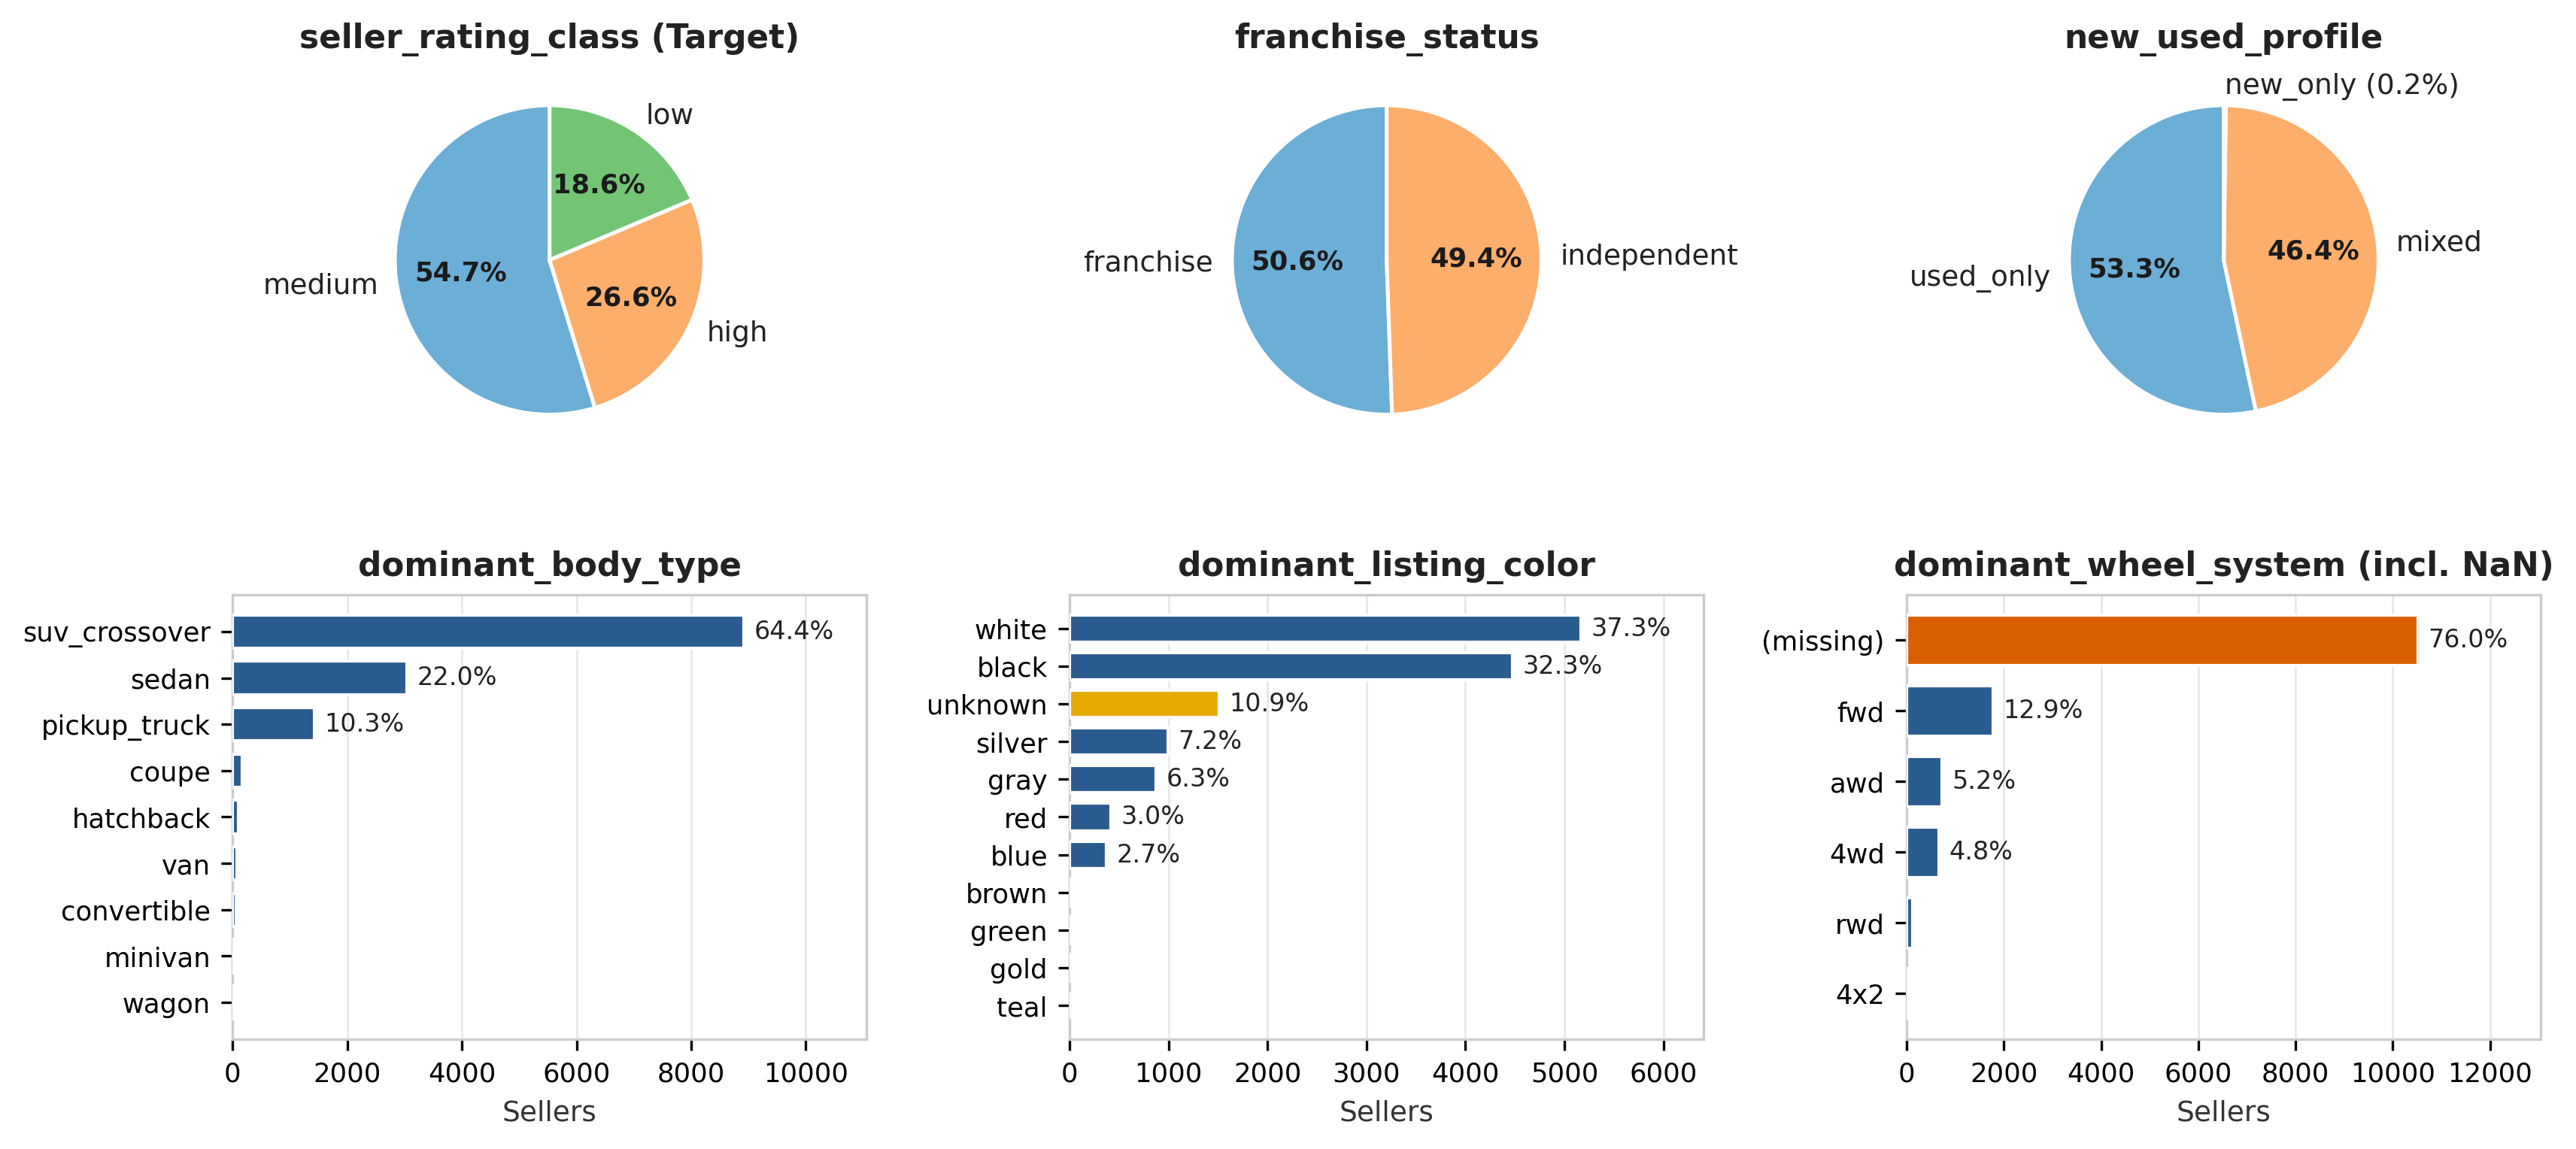
\includegraphics[width=0.98\textwidth]{figures/fig1_2_categorical_combined.png}
  \caption{Distributions of low-cardinality (top) and higher-cardinality (bottom) categorical variables.}
  \label{fig:categorical}
\end{figure}

\subsection{Assessment of data quality}
\label{sec:quality}
A syntactic and semantic audit confirmed that all 13,843 records have unique seller identifiers (\texttt{sp\_id}, converted from \texttt{float64} to \texttt{str} to exclude it from numerical summaries) and zero duplicate rows. All numerical features are non-negative, percentage attributes (\texttt{pct\_*}) lie strictly within $[0, 1]$, discounts never exceed vehicle prices ($\texttt{savings\_amount\_median} < \texttt{price\_median}$), and temporal bounds hold universally ($\texttt{n\_listing\_days} \le \texttt{n\_listings}$ and $\texttt{n\_listing\_days} \le \texttt{listing\_span\_days} + 1$). Half-integer values (\texttt{.5}) observed in count/year medians (\texttt{year\_median}, \texttt{owner\_count\_median}, \texttt{daysonmarket\_median}) are mathematically valid medians of sellers with an even \texttt{n\_listings}.

\subsubsection{Missing value handling}
Across the dataset, 20 attributes contain missing information: 17 columns with explicit \texttt{NaN} entries and 3 categorical columns with implicit \emph{unknown} strings (Table~\ref{tab:missing}). Rather than applying global mean/mode substitution---which would distort multi-segment dealer distributions---we tailored imputation to the missingness mechanism and domain semantics of each attribute group. First, \texttt{dominant\_wheel\_system} was dropped entirely because $75.98\%$ of its records are missing. Second, \texttt{engine\_displacement\_median} ($24.51\%$ missing) was imputed using a two-dimensional stratified median grouped by \texttt{dominant\_body\_type} and \texttt{horsepower\_median} quintiles, preserving the physical coupling between chassis class, engine power, and cylinder volume. Third, for \texttt{dominant\_listing\_color}, the \emph{unknown} label ($10.91\%$) was retained as a distinct category to avoid artificially inflating the modal \emph{white} class, whereas trace \emph{unknown} entries in \texttt{dominant\_transmission} (6 rows) and \texttt{dominant\_fuel\_type} (1 row) were filled via body-type group modes. Finally, the single missing \texttt{vehicle\_age\_median} entry was derived deterministically as $2020 - \texttt{year\_median}$, and the remaining 14 numerical attributes with trace missingness ($<0.30\%$ each, including 3 invalid zeros in \texttt{back\_legroom\_median} recoded as \texttt{NaN}) were imputed using group medians stratified by \texttt{dominant\_body\_type}.

\begin{table}[htbp]
  \centering
  \caption{Summary of explicit (\texttt{NaN}) and implicit (\emph{unknown}) missing values and handling strategies.}
  \label{tab:missing}
  \footnotesize
  \renewcommand{\arraystretch}{0.95}
  \begin{tabular}{p{0.34\linewidth}rrlp{0.36\linewidth}}
    \toprule
    \textbf{Variable / Attribute Group} & \textbf{Missing} & \textbf{Pct (\%)} & \textbf{Type} & \textbf{Handling Strategy} \\
    \midrule
    \texttt{dominant\_wheel\_system} & 10,518 & 75.98\% & \texttt{NaN} & Drop feature ($>50\%$ missing threshold) \\
    \texttt{engine\_displacement\_median} & 3,393 & 24.51\% & \texttt{NaN} & 2D Group median (\texttt{body\_type} $\times$ \texttt{hp\_bin}) \\
    \texttt{dominant\_listing\_color} & 1,510 & 10.91\% & \emph{unknown} & Retain \emph{unknown} as a valid separate category \\
    \texttt{dominant\_transmission}, \texttt{fuel\_type} & 6 / 1 & $\le 0.04\%$ & \emph{unknown} & Group mode by \texttt{dominant\_body\_type} \\
    \texttt{vehicle\_age\_median} & 1 & 0.01\% & \texttt{NaN} & Deterministic formula ($2020 - \texttt{year\_median}$) \\
    14 minor numerical attributes (\texttt{owner\_count\_}, \texttt{pct\_*}, dimensions, legrooms, fuel economy, \texttt{horsepower\_}, \texttt{mileage\_}) & 1--39 each & 0.01--0.28\% & \texttt{NaN} & Group median by \texttt{dominant\_body\_type} (incl.\ 3 zero-legroom noise records $\rightarrow$ \texttt{NaN}) \\
    \bottomrule
  \end{tabular}
\end{table}

\subsubsection{Outlier and noise detection}
Inspection of the feature distributions (Figure~\ref{fig:boxplots}) distinguishes physical measurement errors from legitimate market extremes:
\begin{itemize}
  \item \textbf{True semantic noise:} Exactly 3 records report $\texttt{back\_legroom\_median} = 0$ despite having \texttt{suv\_crossover} or \texttt{sedan} as their \texttt{dominant\_body\_type}. Since zero rear legroom is physically impossible for multi-row passenger vehicles, these entries were recoded as \texttt{NaN} and imputed via body-type group medians.
  \item \textbf{Valid domain outliers:} For sparse risk indicators (\texttt{pct\_salvage} and \texttt{pct\_theft\_title}, with $90.83\%$ and $84.56\%$ zeros), $\text{IQR} = 0$ causes standard Tukey fences to flag any non-zero dealer as an outlier. Similarly, extreme right-tail values across continuous features reflect genuine niche dealerships rather than noise: high-volume aggregators (\texttt{n\_listings} up to 4,959), luxury/classic specialists (\texttt{price\_median} up to \$236,438, \texttt{horsepower\_median} up to 630 HP, \texttt{vehicle\_age\_median} up to 60 years), electric-vehicle dealers (\texttt{city\_fuel\_economy\_median} up to 126 MPG), and slow-turnover lots (\texttt{daysonmarket\_median} up to 1,987 days). All 13,843 records were therefore retained to preserve market representation, while tail leverage is mitigated via logarithmic transformation in Section~\ref{sec:transformation}.
\end{itemize}

\begin{figure}[htbp]
  \centering
  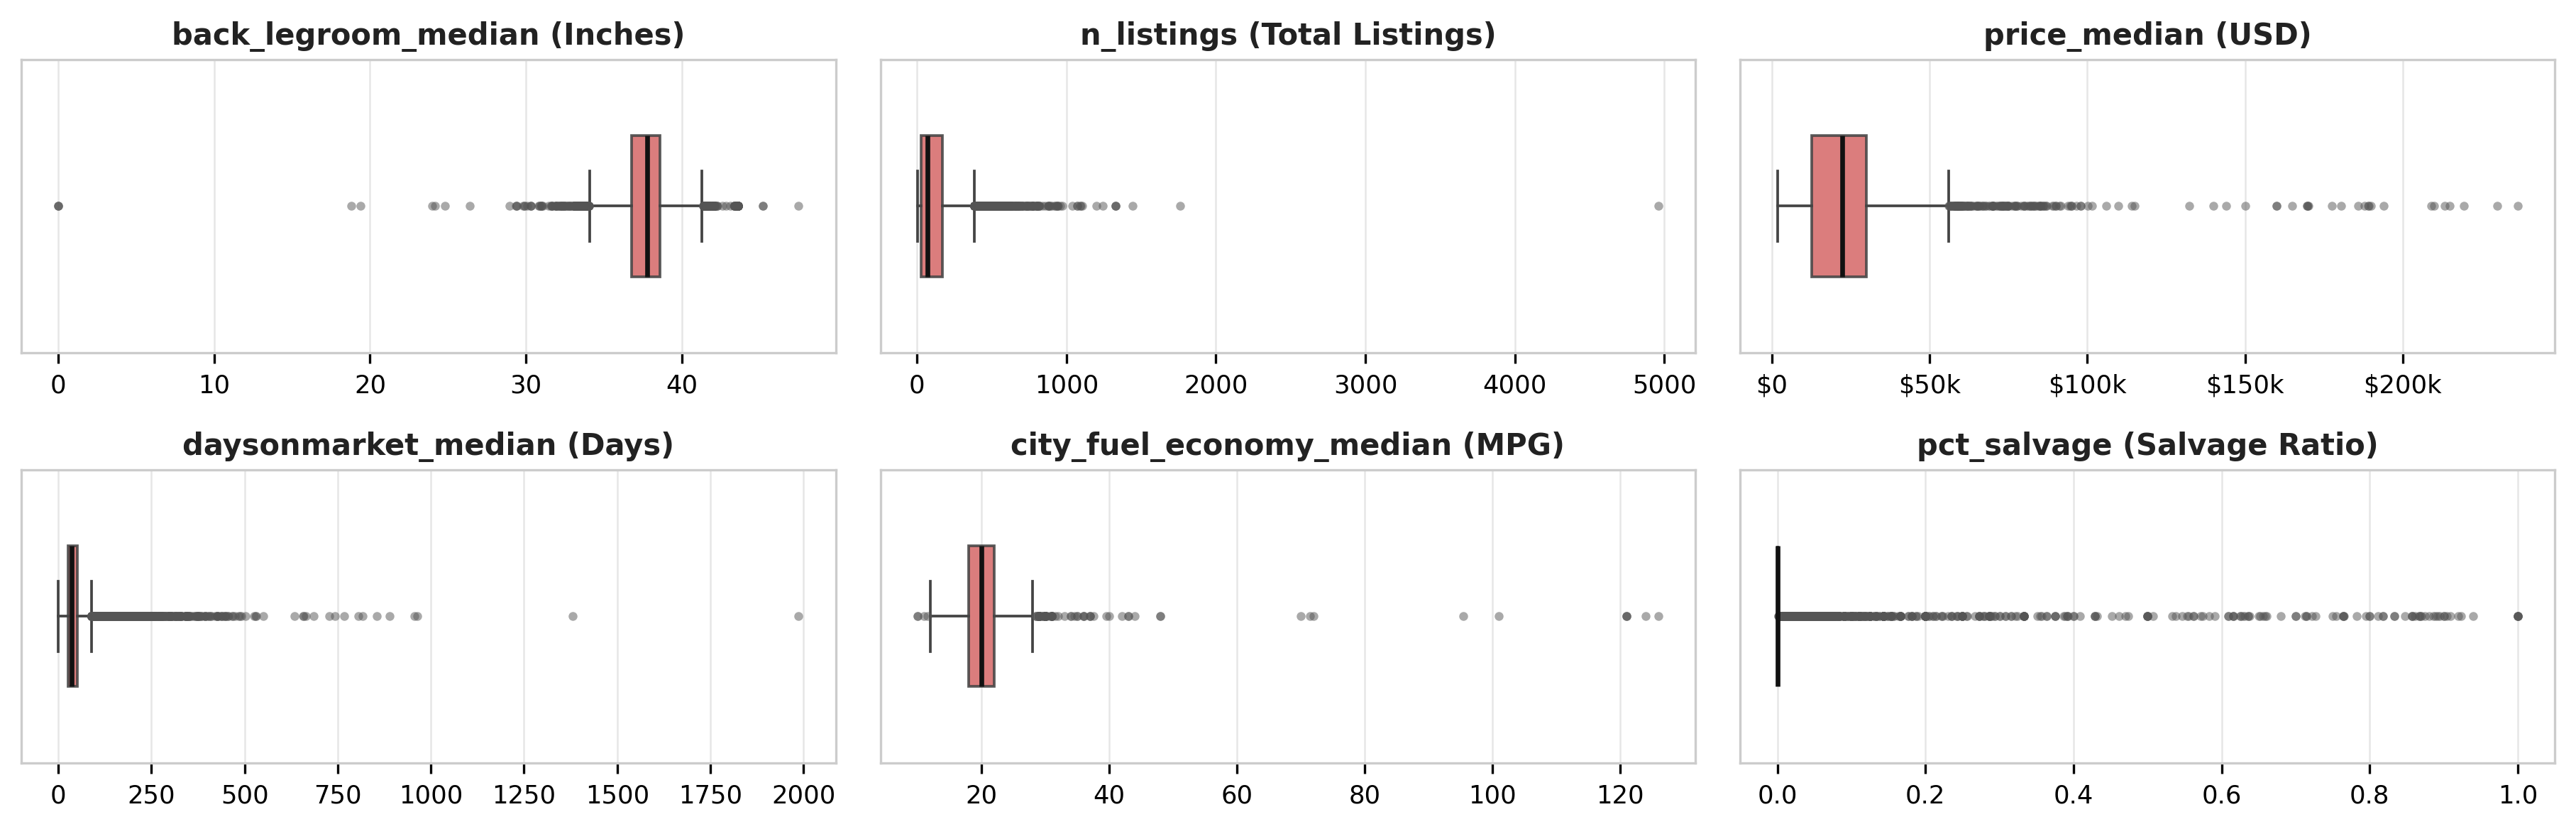
\includegraphics[width=0.96\textwidth]{figures/fig1_3_boxplots_outliers_compact.png}
  \caption{Representative boxplots illustrating true semantic noise (\texttt{back\_legroom\_median = 0}) versus valid domain outliers and $\text{IQR}=0$ zero-inflated ratios.}
  \label{fig:boxplots}
\end{figure}

\subsubsection{Variables transformation}
\label{sec:transformation}
To mitigate the extreme right skewness ($\text{Skewness} > 1$) identified in Section~\ref{sec:distribution} without discarding valid niche dealerships, we applied the zero-safe logarithmic transformation $\log(1 + x)$ to the nine heavily skewed continuous attributes (\texttt{n\_listings}, \texttt{price\_median}, \texttt{savings\_amount\_median}, \texttt{daysonmarket\_median}, \texttt{vehicle\_age\_median}, \texttt{engine\_displacement\_median}, \texttt{city\_fuel\_economy\_median}, \texttt{highway\_fuel\_economy\_median}, and \texttt{fuel\_tank\_volume\_median}), compressing heavy right tails into near-symmetric distributions. Because numerical attributes span incompatible units, we subsequently exported two scaled master representations for downstream modelling: \textbf{Z-score standardisation} ($\mu=0, \sigma=1$) and \textbf{Min-Max normalisation} ($[0, 1]$).

\subsubsection{Pairwise correlations and variable elimination}
\label{sec:correlations}

\noindent
\begin{minipage}[t]{0.46\textwidth}
  \vspace{0pt}
  Inter-feature dependencies were evaluated using a sampled pairwise regression plot matrix (Figure~\ref{fig:pairplot}) and the full Spearman rank correlation matrix (Figure~\ref{fig:spearman}). Spearman's $\rho$ was chosen over Pearson's $r$ because the bivariate distributions exhibit strong non-linear monotonic trajectories alongside heavy tails---most notably the L-shaped depreciation curve where \texttt{price\_median} decays steeply with \texttt{mileage\_median} ($\rho = -0.82$) and \texttt{vehicle\_age\_median} ($\rho = -0.82$) before plateauing, which linear regression lines fail to capture.
  
  \medskip
  The correlation structure reveals three main domain blocks and guides redundancy elimination:
  \begin{itemize}
    \item \textbf{Powertrain trade-offs:} \texttt{engine\_displacement\_median} correlates strongly with \texttt{fuel\_tank\_volume\_median} ($\rho = 0.79$) and \texttt{horsepower\_median} ($\rho = 0.76$), and inversely with \texttt{city\_fuel\_economy\_median} ($\rho = -0.76$), capturing the physical trade-off between engine capacity and fuel efficiency.
  \end{itemize}
\end{minipage}\hfill
\begin{minipage}[t]{0.51\textwidth}
  \vspace{0pt}
  \centering
  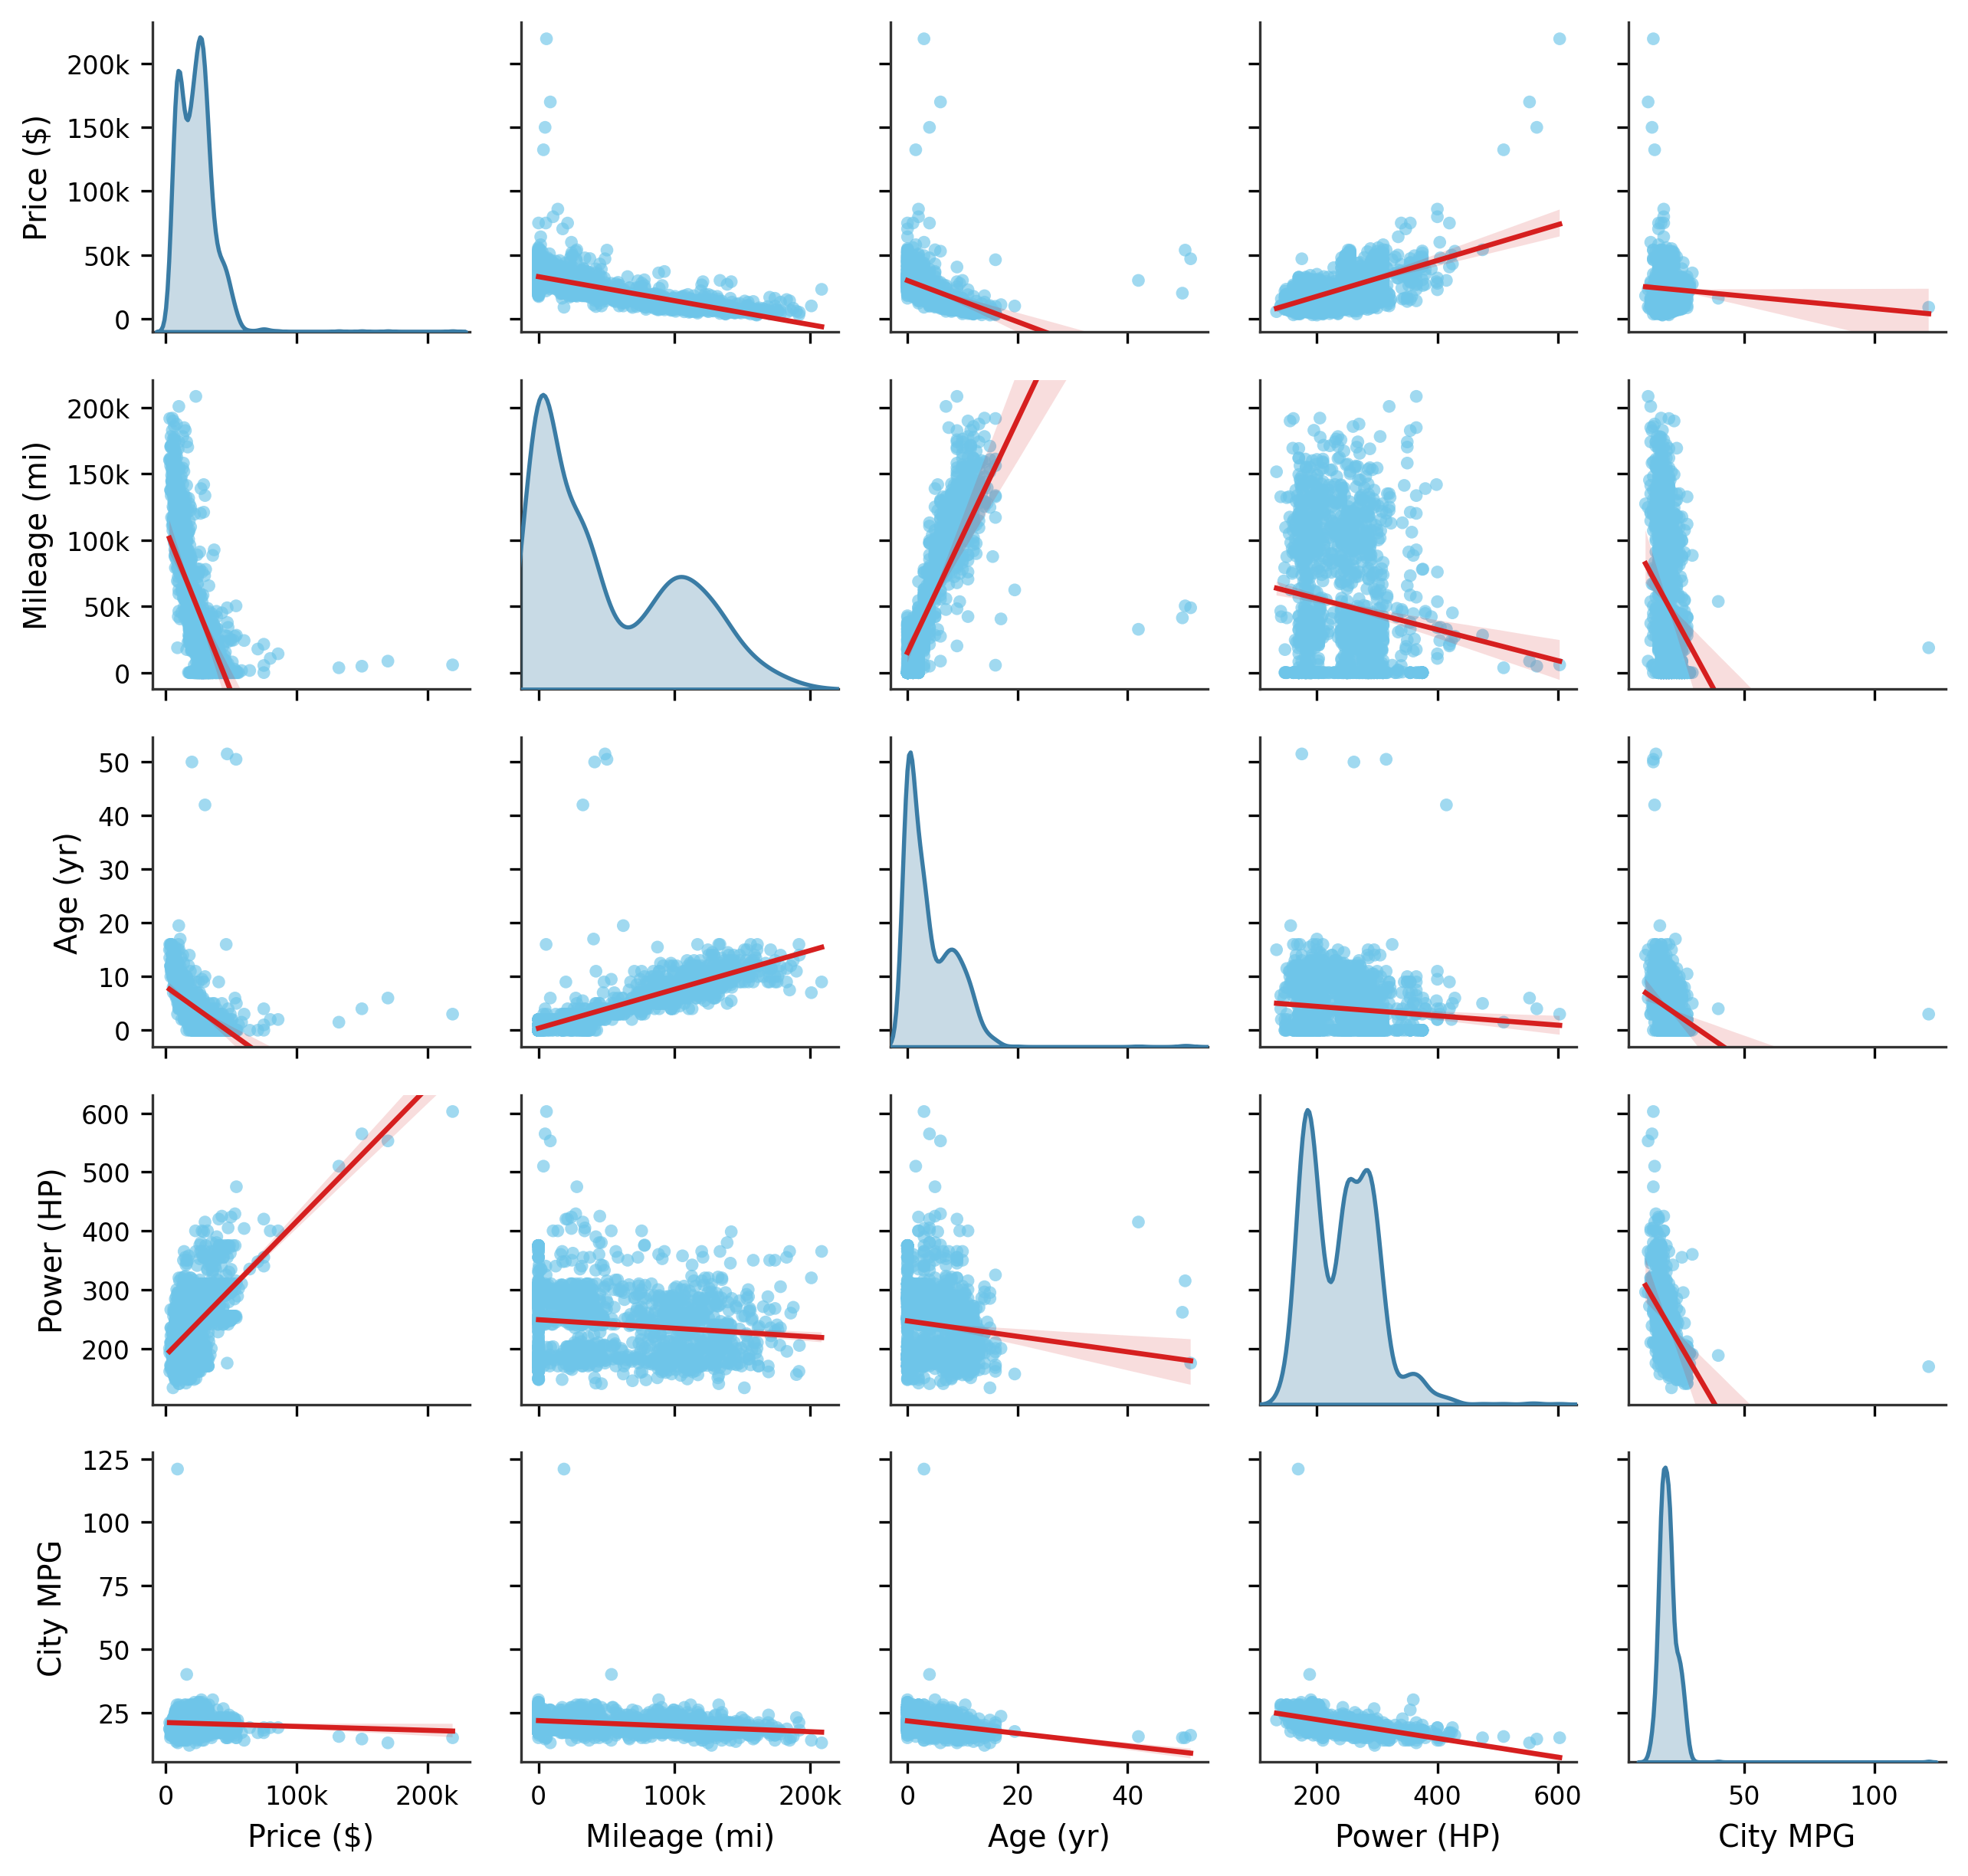
\includegraphics[width=\linewidth]{figures/fig1_4_pairplot_compact.png}
  \captionof{figure}{Pairwise regression plot matrix of four core numerical attributes (sampled $n=1,500$).}
  \label{fig:pairplot}
\end{minipage}

\medskip
\noindent
\begin{minipage}[t]{0.54\textwidth}
  \vspace{0pt}
  \centering
  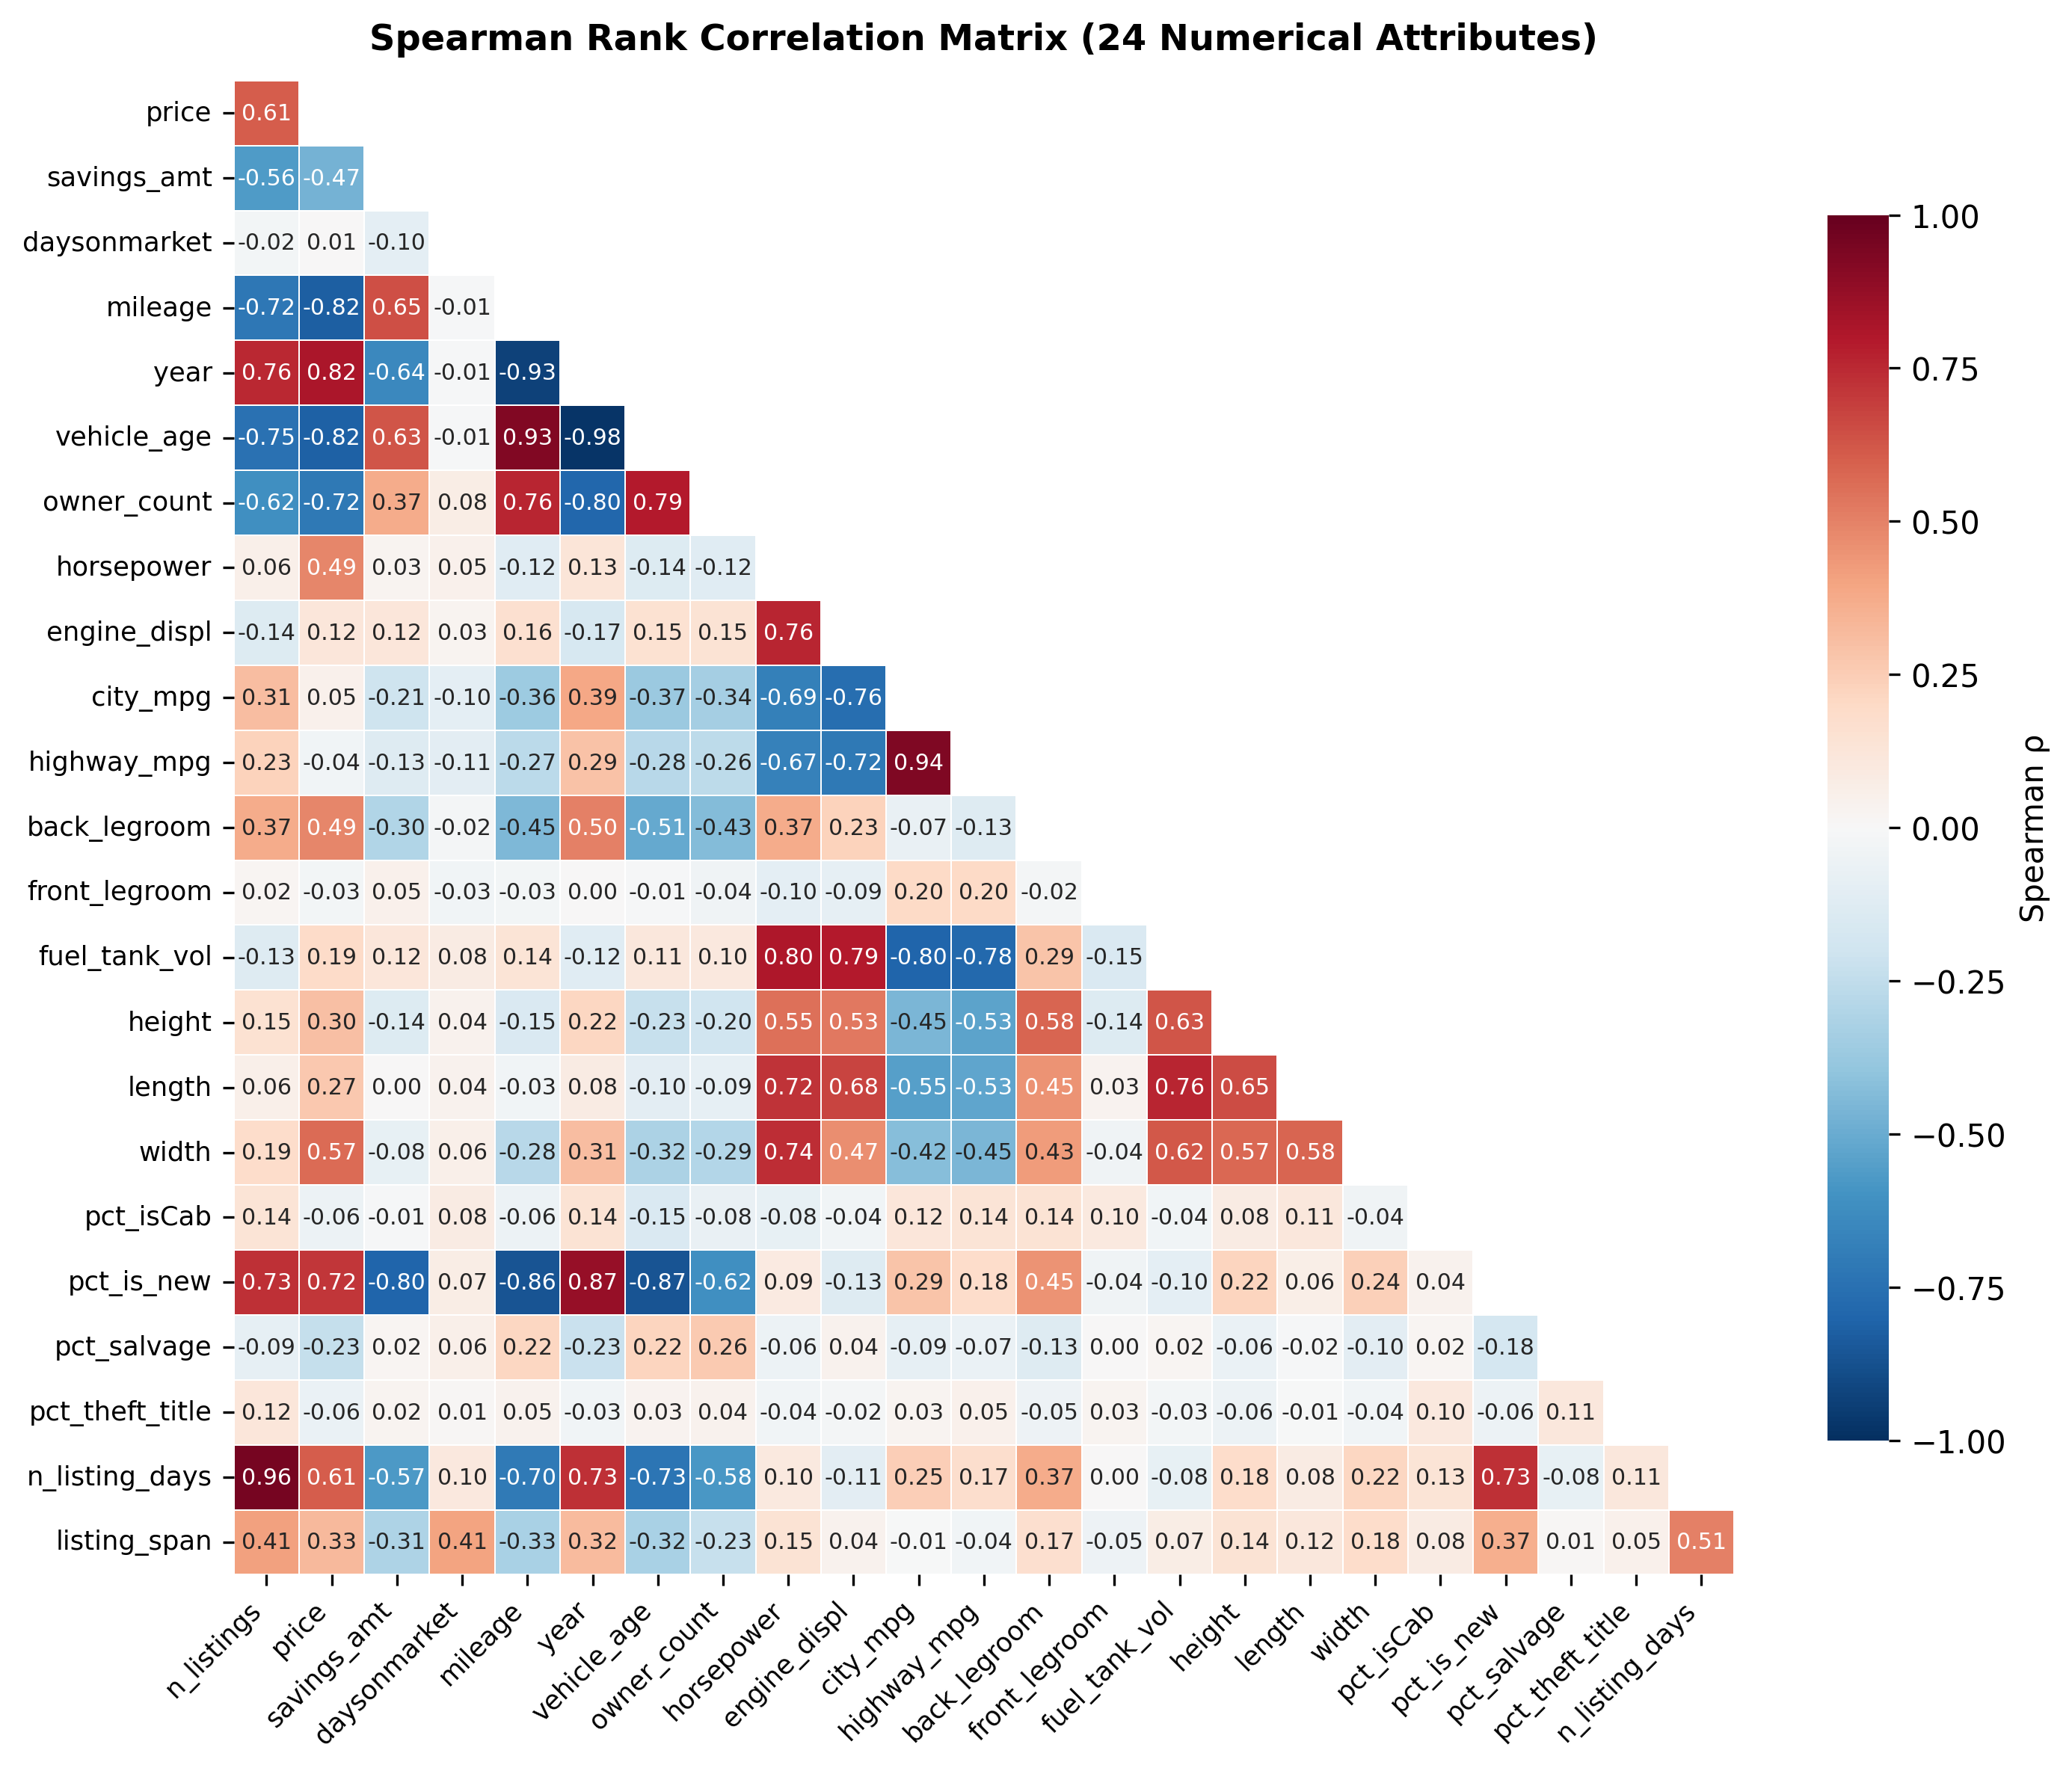
\includegraphics[width=\linewidth]{figures/fig1_5_spearman_heatmap_compact.png}
  \captionof{figure}{Spearman rank correlation matrix across the 24 numerical attributes.}
  \label{fig:spearman}
\end{minipage}\hfill
\begin{minipage}[t]{0.43\textwidth}
  \vspace{0pt}
  \begin{itemize}
    \item \textbf{Collinear pairs retained for ratio engineering:} Although \texttt{mileage\_median} and \texttt{vehicle\_age\_median} ($\rho = 0.93$) as well as \texttt{n\_listings} and \texttt{n\_listing\_days} ($\rho = 0.96$) are strongly collinear, both pairs were retained in the master dataset because their relative ratios define annual utilisation intensity ($\texttt{mileage} / \texttt{age}$) and daily posting velocity ($\texttt{listings} / \texttt{active\_days}$) in downstream tasks.
    \item \textbf{Redundant feature elimination:} We removed \texttt{year\_median} ($\rho = -0.98$ with \texttt{vehicle\_age\_median}, being an exact linear shift $2020 - \texttt{year\_median}$) and \texttt{highway\_fuel\_economy\_median} ($\rho = 0.94$ with \texttt{city\_fuel\_economy\_median}, capturing duplicate fuel-efficiency information). Combined with the exclusion of the identifier \texttt{sp\_id} and \texttt{dominant\_wheel\_system}, the final prepared dataset comprises \textbf{13,843 records and 29 attributes} (22 numerical and 7 categorical).
  \end{itemize}
\end{minipage}
